\section{Benchmark Suite} 
\label{sec:mavbench}

\begin{figure*}[t]
\centering
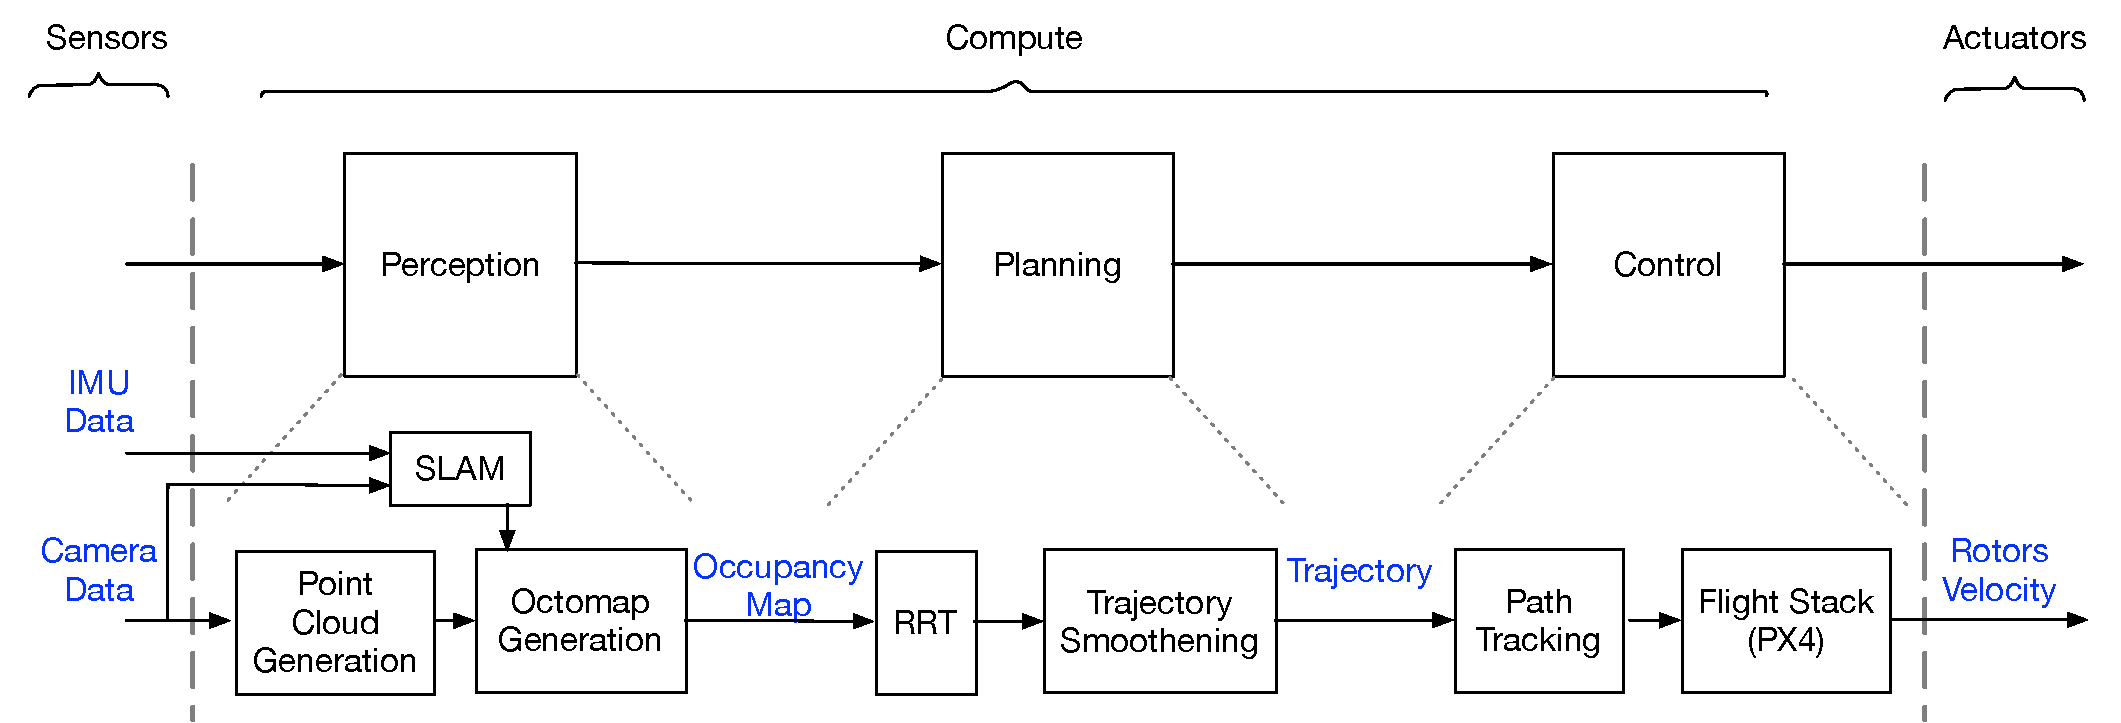
\includegraphics[height=1.65in, keepaspectratio]{figs/software_pipeline}
\caption{High-level application pipeline for a typical MAV application. The upper row presents a universal pipeline that all our MAVBench applications follow, which involves \emph{perception}, \emph{planning} and \emph{control}. The lower row presents how a specific workload in MAVBench (e.g. package delivery) maps to the universal high-level application pipeline.}
\label{fig:software_pipeline}
\end{figure*}


To quantify the power and performance demands of typical MAV applications, we created a set of workloads that we compiled into a benchmark suite. Our benchmarks run on top of our closed-loop simulation environment. The suite aims to cover a wide range of representative applications. Each workload is an \textit{end-to-end} application that allows us to study the kernels' impact on the whole application as well as to investigate the interactions and dependencies between kernel. 

By providing holistic end-to-end applications instead of only focusing on individual kernels, MAVBench allows for the examination of kernels' impacts and their optimization at the application level. This is a lesson learned from Amdahl's law, which recognizes that the true impact of a component's improvement needs to be evaluated globally rather than locally.

In \Sec{sec:sw_pipeline}, we present a high level software pipeline associated (though not exclusive) to our workloads. In \Sec{sec:benchmarks}, we present functional summaries of the workloads in MAVBench, their use cases, and mappings from each workload to the high level software pipeline. In \Sec{sec:kernels}, we describe in details of the prominent computational kernels that are incorporated into our workloads, and finally in \Sec{sec:QoF} we provide a short discussion regarding the Quality-of-Flight (QoF) metrics to evaluate MAV applications.

The MAVBench workloads have different computational kernels, as shown in Table~\ref{kernel_makeup}. MAVBench aims at being comprehensive by (1) selecting applications that target different robotic domains (robotics in hazardous areas, construction, etc.) and (2) choosing kernels (e.g. point cloud, RRT) common across a range of applications, not limited to our benchmark-suite. The computational kernels (OctoMaps, RTT, etc.) that we use in the benchmarks are the building blocks of many robotics applications and hence they are platform agnostic. 

% Our insights carry over to rotorcraft UAVs and AUVs (Autonomous underwater vehicles), since in both cases constant power is required to maintain the position. Furthermore, ground mobile robots under high energy constraints can also exploit principles presented.


% Application architecture section
% Add low-level details like which kernels we use
% Mention that we have flexibility
% Add small details like SLAM-backtracking, Octomap, ROS
% Add new paragraphs after every benchmark
% Some analysis of benchmarks (length of runtime, number of ROS nodes)
% Literature survey (PARSEC, BioBench, WHISPER)
% Add annotated graphics to system architecture showing sensors
% Draw an end-to-end diagram or a table
% Talk about core kernels to foreshadow future characterization


\subsection{Application Dataflow} \label{sec:sw_pipeline}

\begin{figure*}[t]
	\centering
	\begin{subfigure}[t]{1.385in}
		\centering
		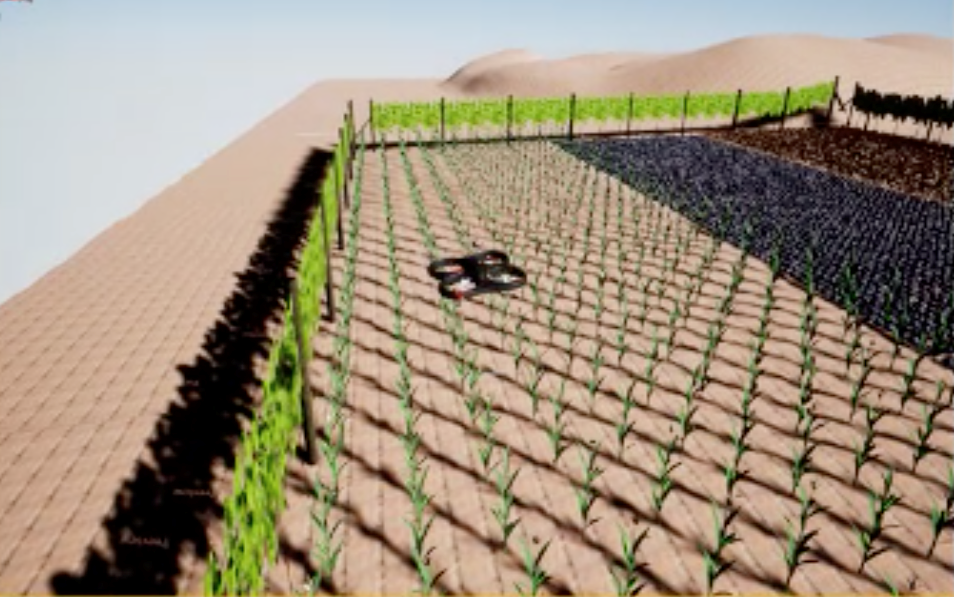
\includegraphics[width=\textwidth, height=1in]{figs/benchmarks/scanning}
		\caption{Scanning.}\label{fig:benchmarks:scanning}
	\end{subfigure}
	\hfill
	\begin{subfigure}[t]{1.385in}
		\centering
		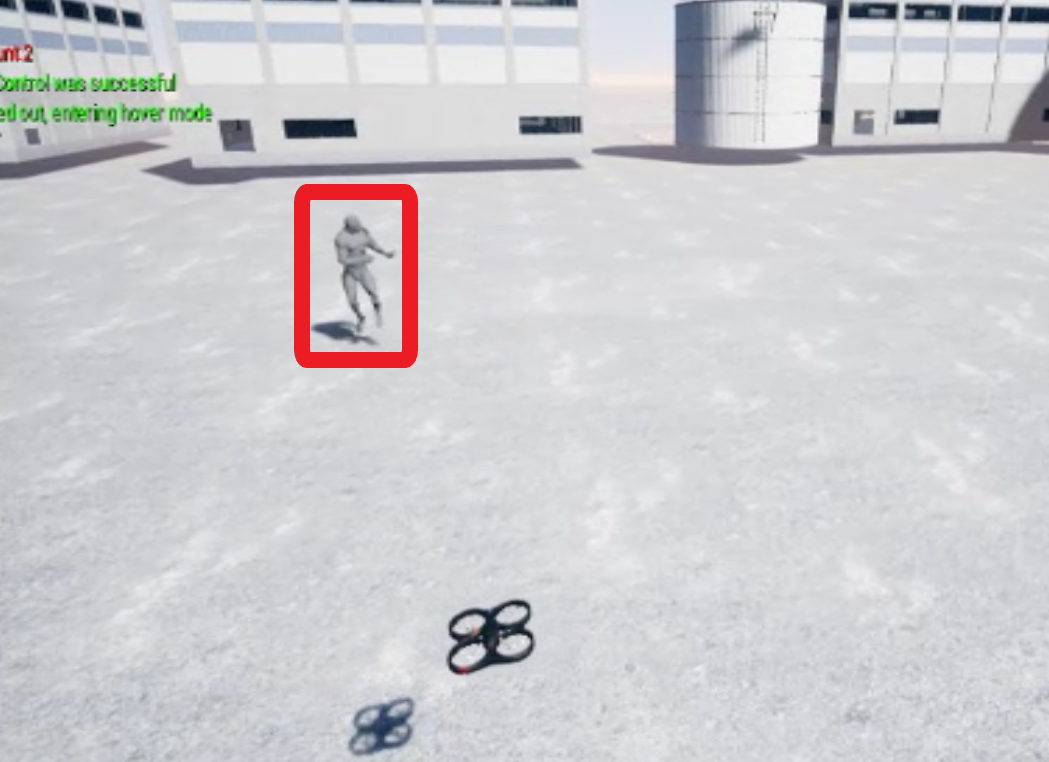
\includegraphics[width=\textwidth, height=1in]{figs/benchmarks/aerial-photo}
		\caption{Aerial Photography.}\label{fig:benchmarks:aerial-photo}
	\end{subfigure}
	\hfill
    \begin{subfigure}[t]{1.385in}
		\centering
		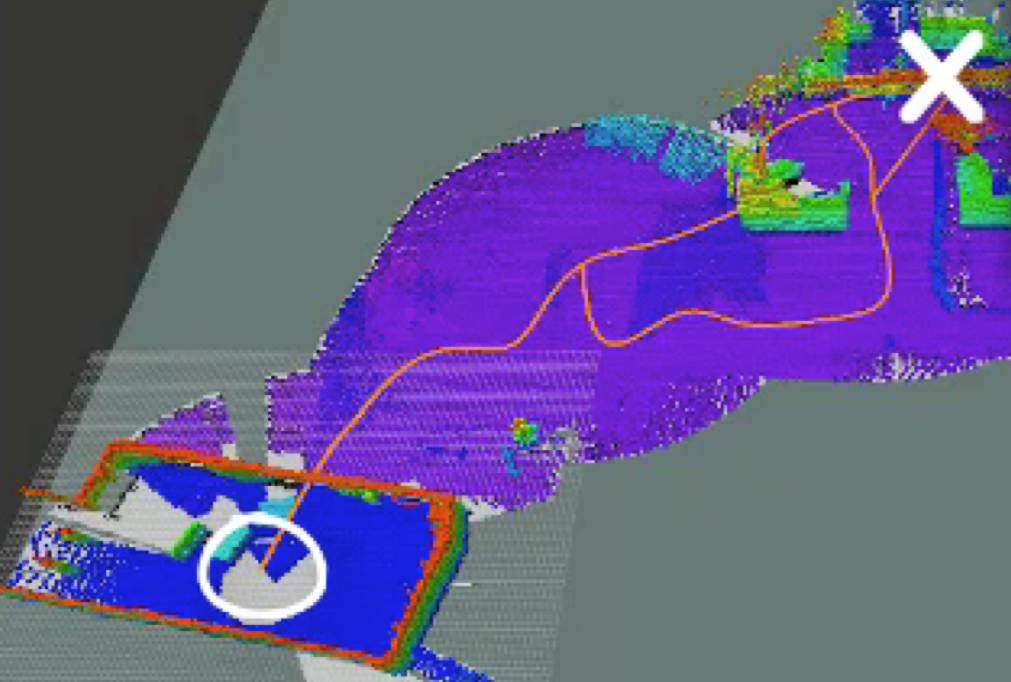
\includegraphics[width=\textwidth, height=1in]{figs/benchmarks/package-delivery}
		\caption{Package Delivery.}\label{fig:benchmarks:package-delivery}
	\end{subfigure}
	\hfill
    \begin{subfigure}[t]{1.385in}
		\centering
		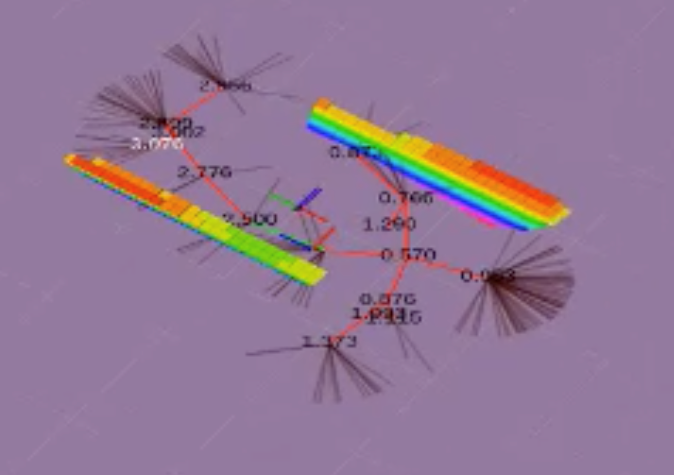
\includegraphics[width=\textwidth, height=1in]{figs/benchmarks/3d-mapping}
		\caption{3D Mapping.}\label{fig:benchmarks:3D-mapping}
	\end{subfigure}
	\hfill
    \begin{subfigure}[t]{1.385in}
		\centering
		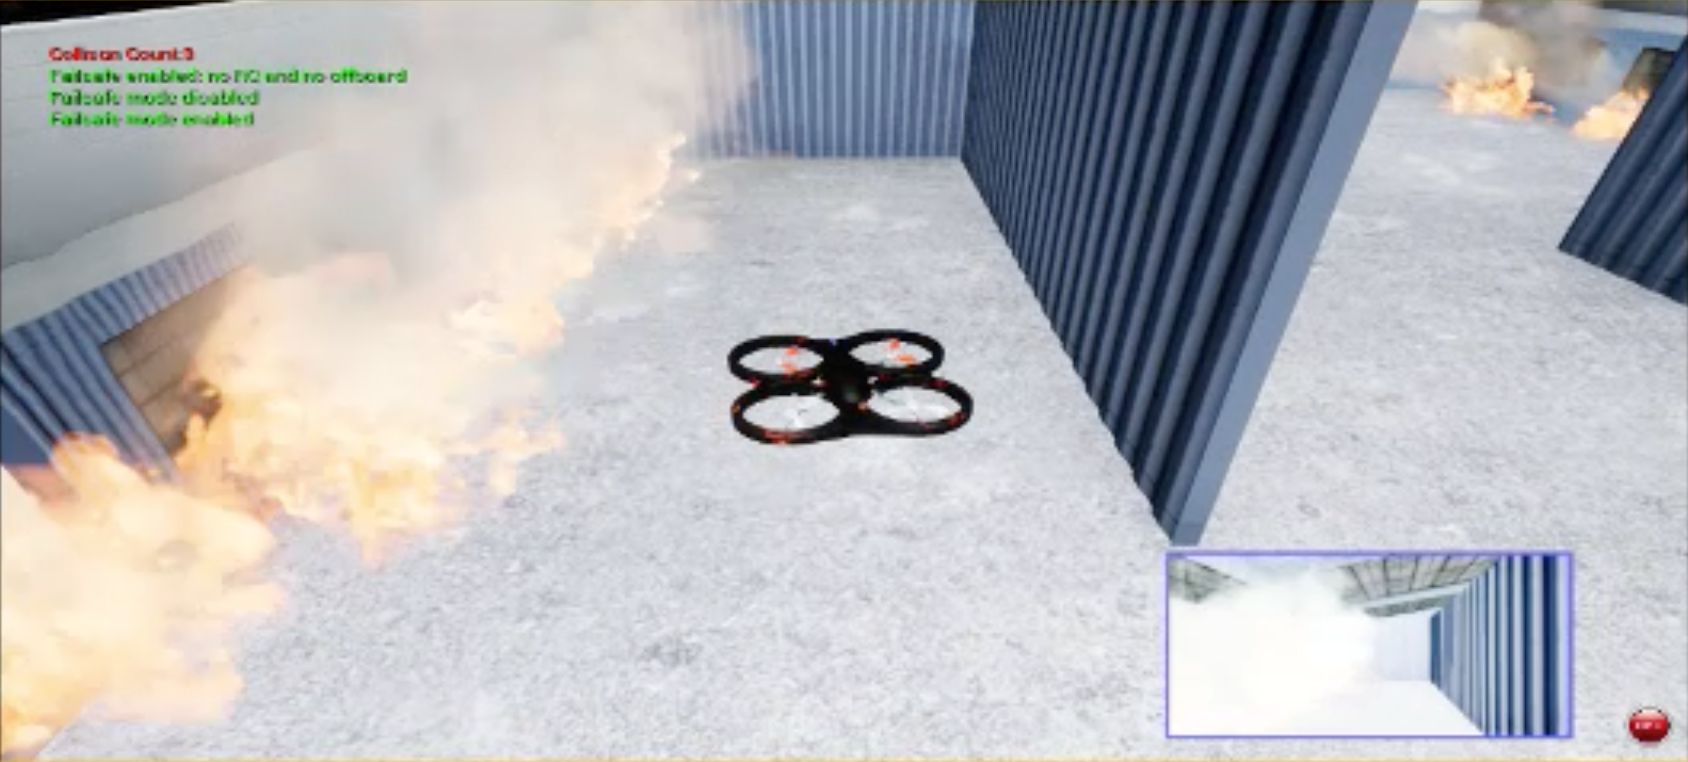
\includegraphics[width=\textwidth, height=1in]{figs/benchmarks/search-and-rescue}
        \caption{Search and Rescue.}\label{fig:benchmarks:search-and-rescue}
	\end{subfigure}
    \vspace{-5pt}
    \caption{MAVBench workloads. Each workload is an end-to-end application targeting both industry and research use cases. All figures are screenshots of a MAV executing a workload within its simulated environment. Fig.~\ref{fig:benchmarks:package-delivery} shows a MAV planning a trajectory to deliver a package. Fig.~\ref{fig:benchmarks:3D-mapping} shows a MAV sampling its environment in search of unexplored areas to map.}
    \label{fig:bench_screenshot}
\end{figure*}

\begin{figure}[t!]
	\centering
	\begin{subfigure}[t]{\columnwidth}
		\centering
        \vspace{-5pt}
		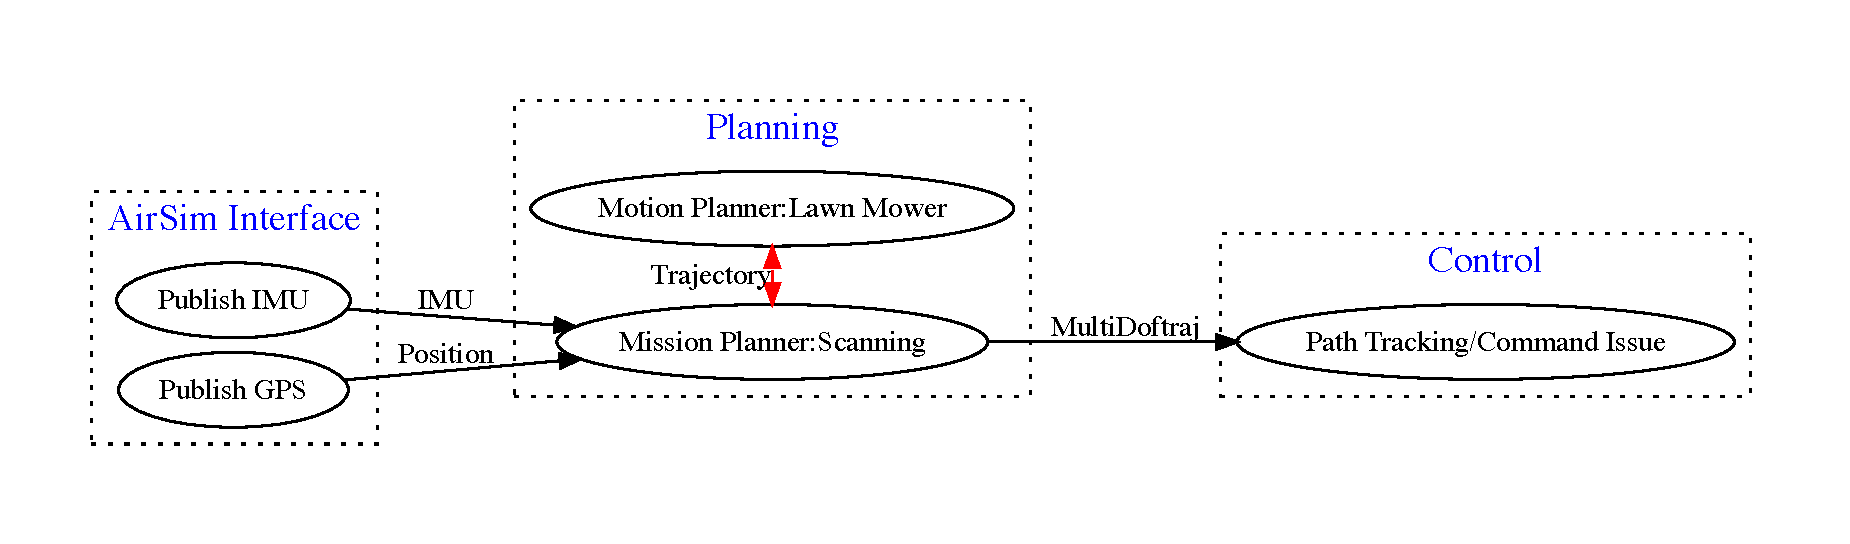
\includegraphics[width=\columnwidth]{figs/data_flow/scanning}
        \vspace{-20pt}
\caption{Scanning.}\label{fig:benchmarks:data-flow:scanning}
	\end{subfigure}
    %\vspace{-10pt}
    \begin{subfigure}[t]{\columnwidth}
		\centering
		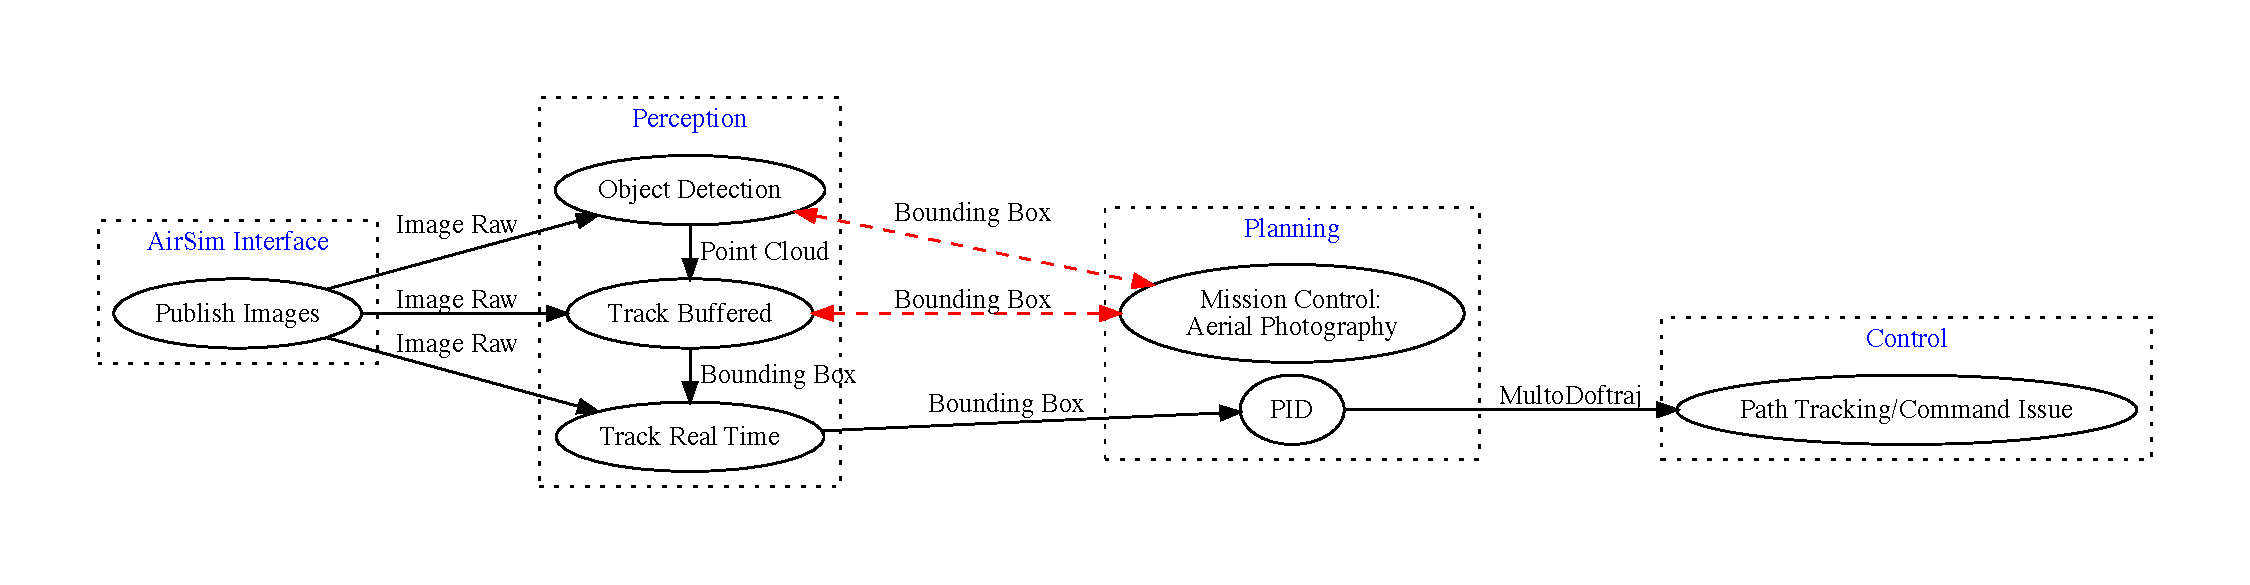
\includegraphics[width=\columnwidth]{figs/data_flow/aerial_photography}
        \vspace{-20pt}
		\caption{Aerial Photography.}\label{fig:benchmarks:data-flow:aerial_photography}
	\end{subfigure}
    %\vspace{-10pt}
	\begin{subfigure}[t]{\columnwidth}
		\centering
		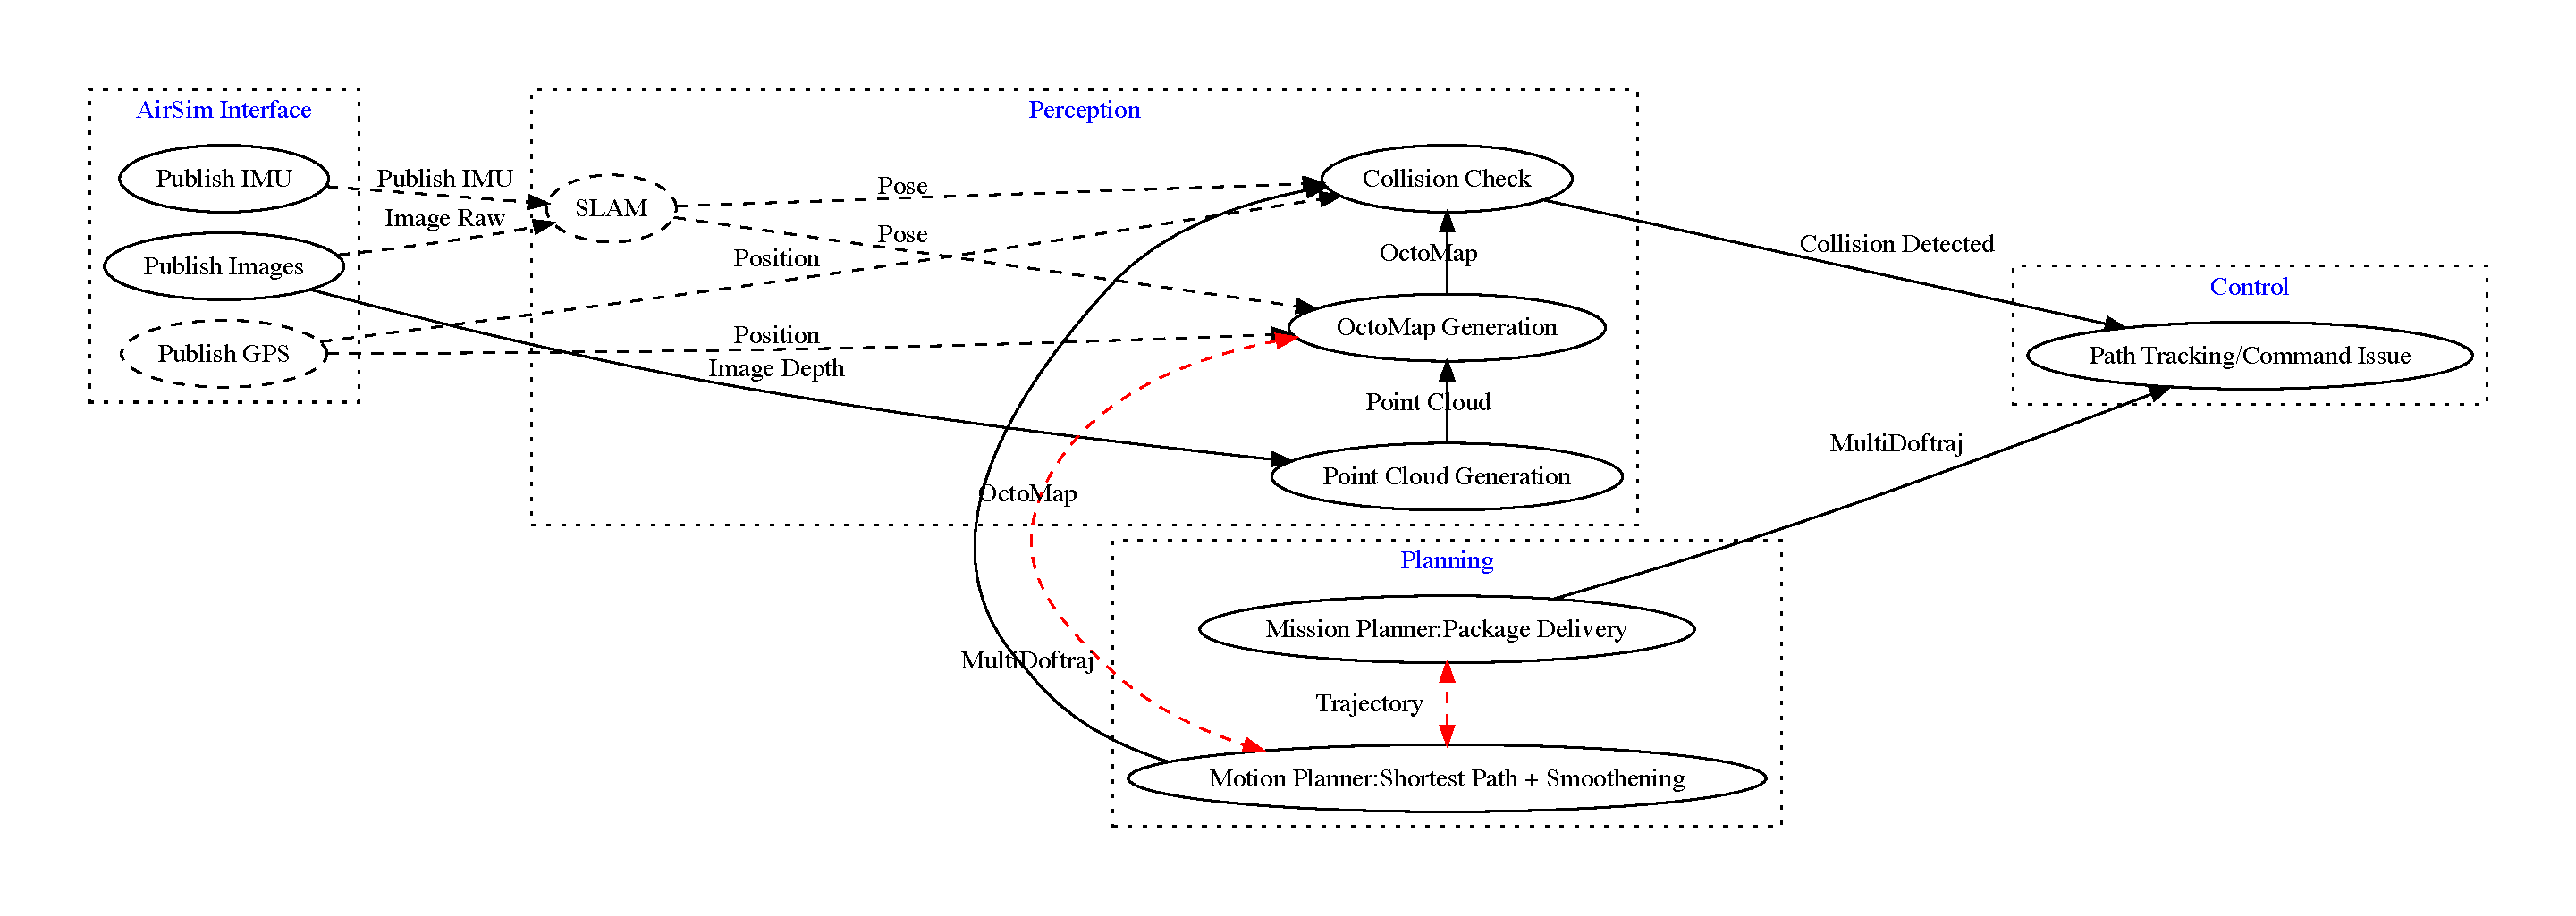
\includegraphics[width=\columnwidth] {figs/data_flow/package_delivery}
        \vspace{-20pt}
		\caption{Package Delivery.}\label{fig:benchmarks:data-flow:package_deilvery}
	\end{subfigure}
    %\vspace{-10pt}
    \begin{subfigure}[t]{\columnwidth}
		\centering
		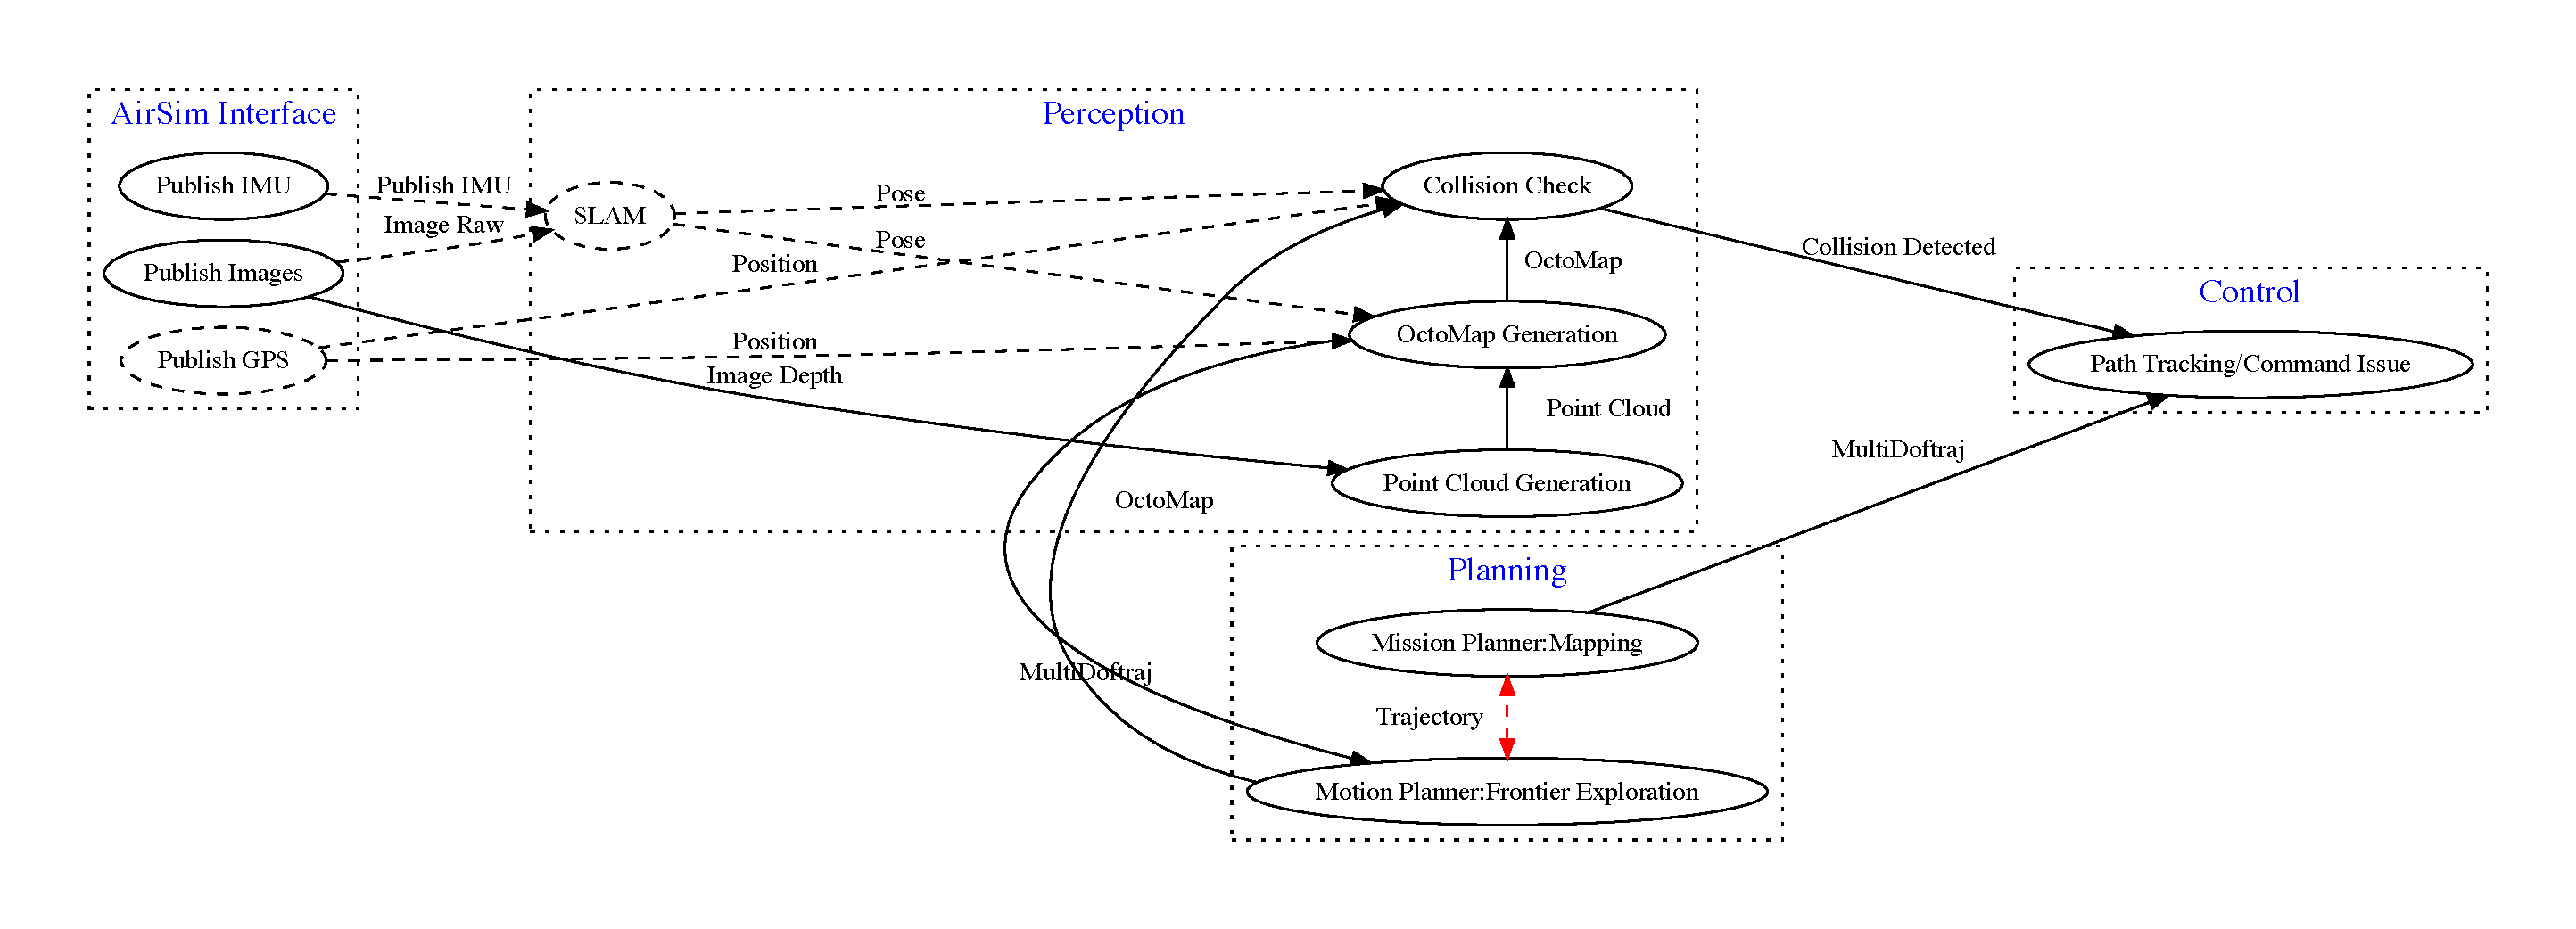
\includegraphics[width=\columnwidth]{figs/data_flow/mapping}
        \vspace{-20pt}
		\caption{3D Mapping.}\label{fig:benchmarks:data-flow:mapping}
	\end{subfigure}
    %\vspace{-10pt}
    \begin{subfigure}[t]{\columnwidth}
		\centering
		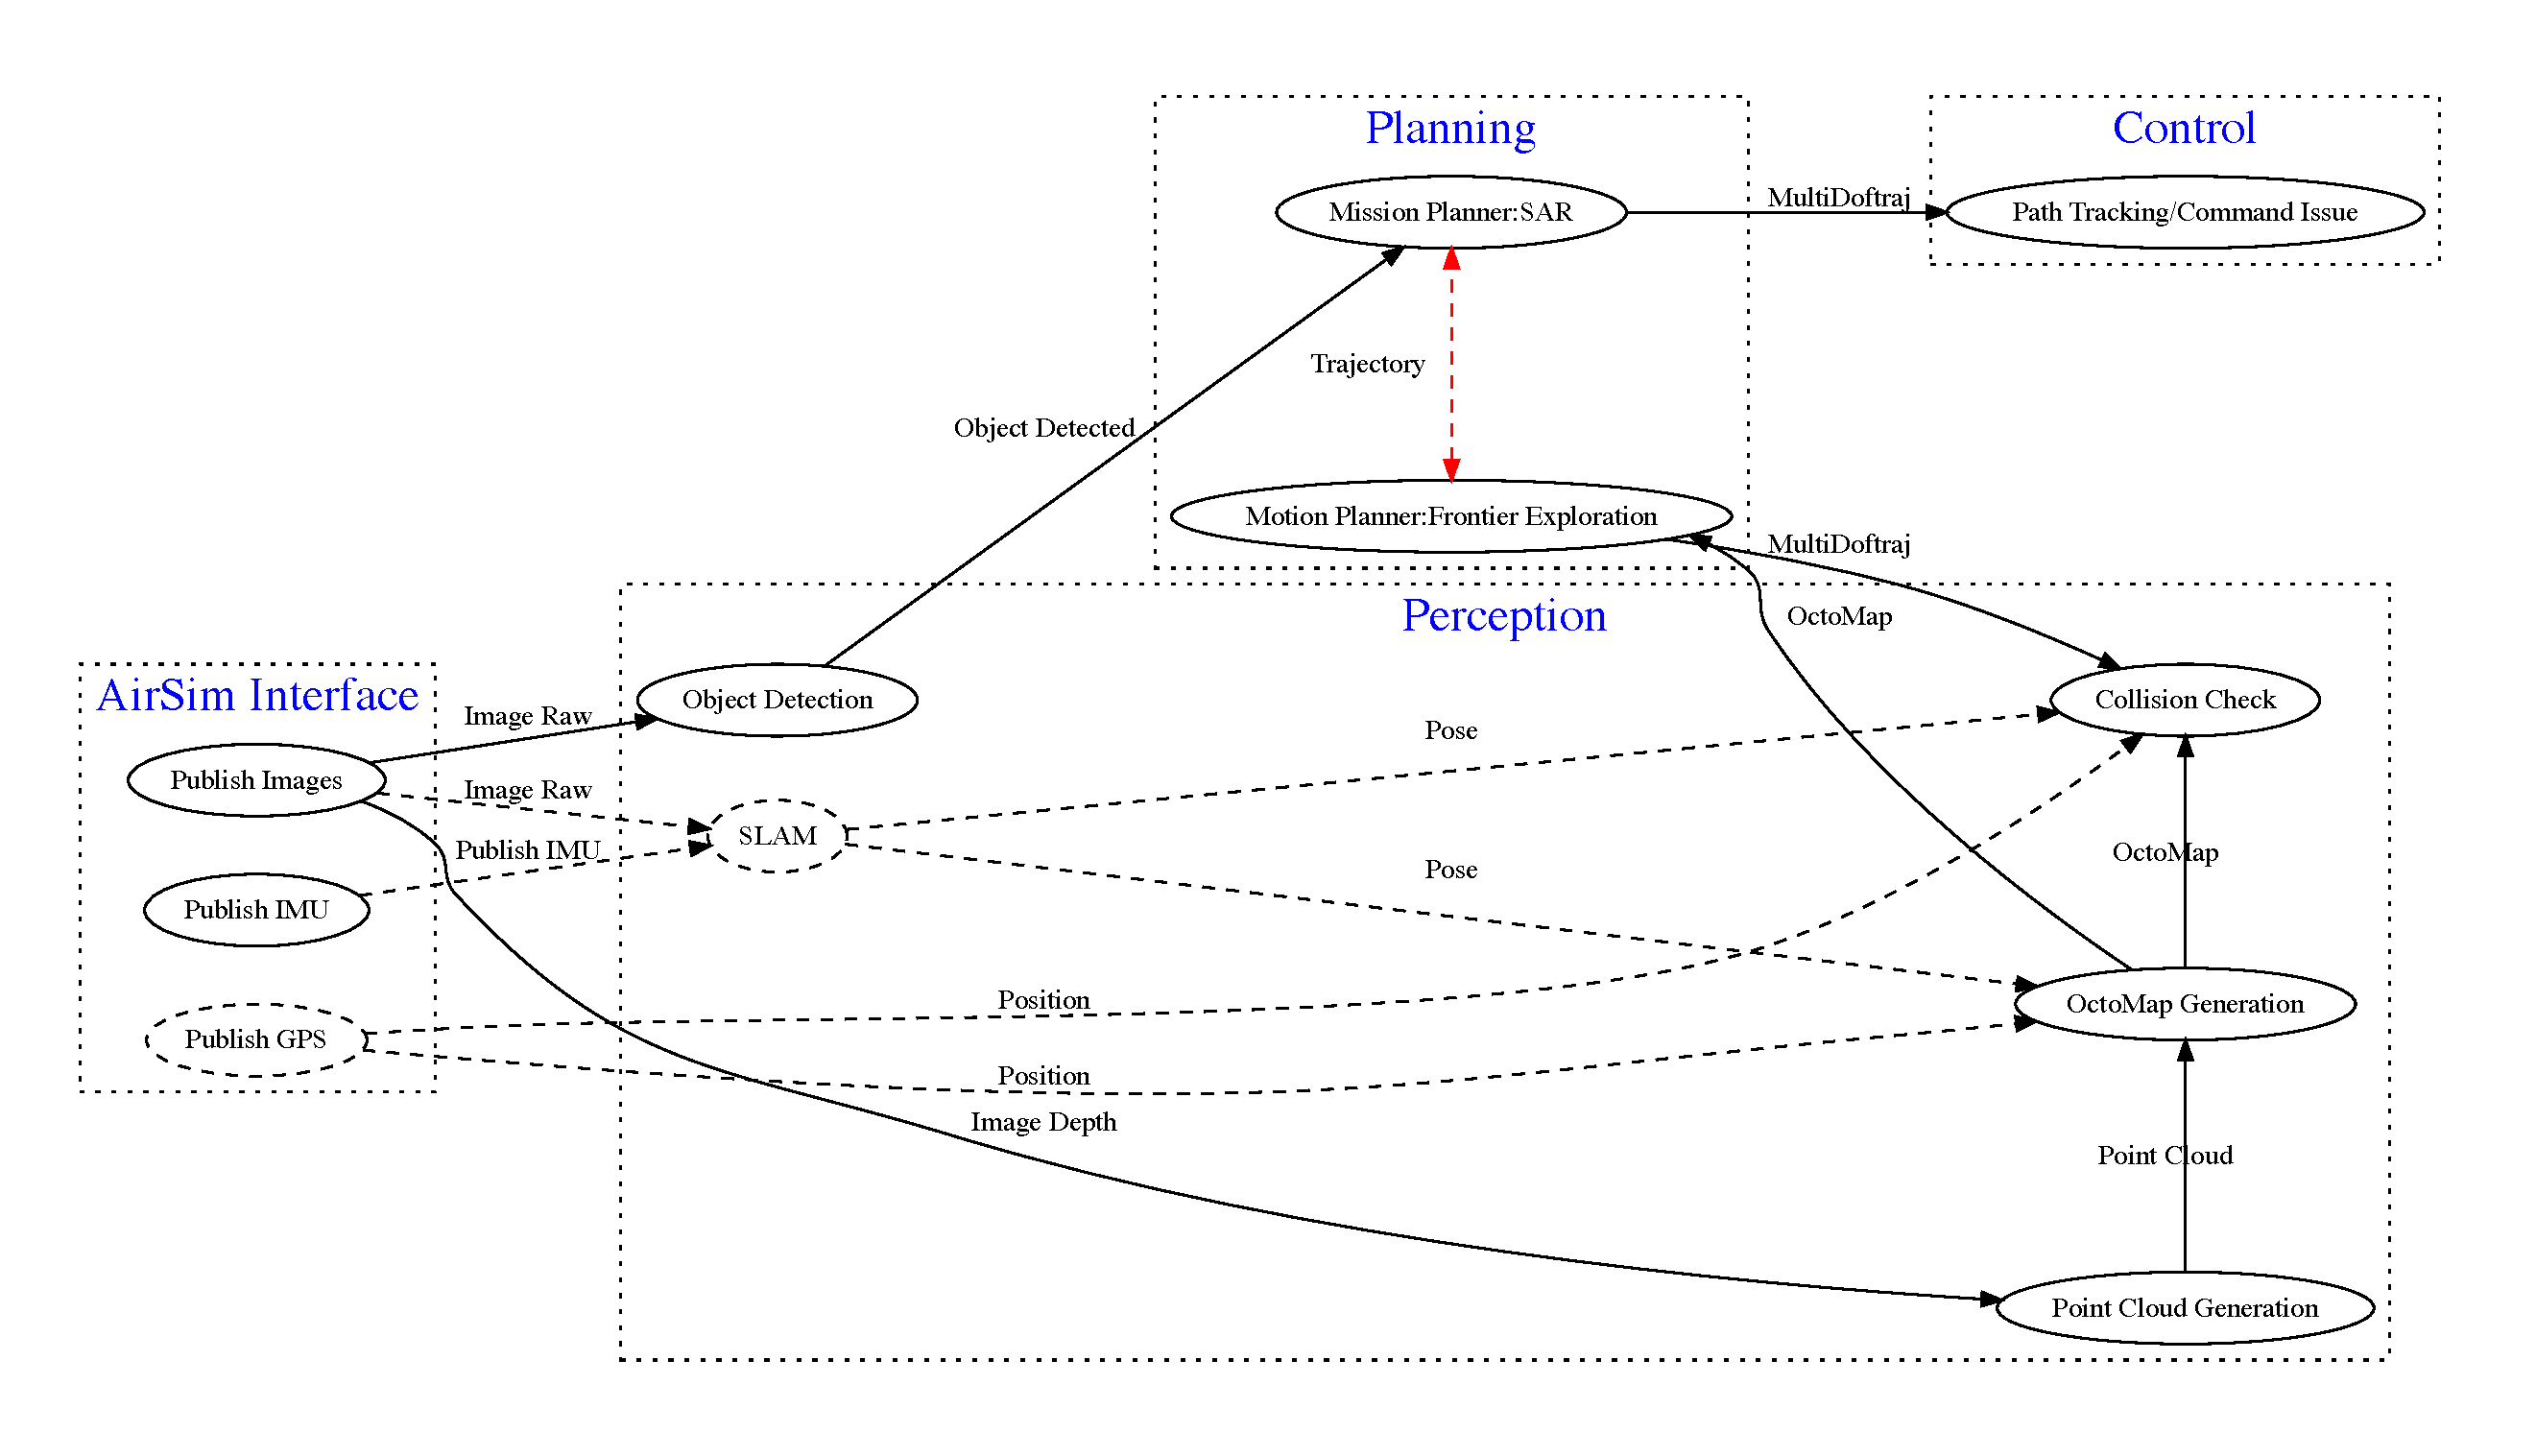
\includegraphics[width=\columnwidth]{figs/data_flow/sar}
        %\vspace{-20pt}
		\caption{Search and Rescue.}\label{fig:benchmarks:data-flow:sar}
	\end{subfigure}
    \caption{Application dataflows. Nodes are denoted with a circle and communication between the nodes is captured with an arrow. If the communication paradigm between the nodes is of a subscriber/publisher kind, the arrows are filled and black, whereas in the case of the client/server paradigm, they are dotted and red. Nodes with a subscriber/publisher communication paradigm or without any at all run in parallel. Dotted lines denote various localization techniques.}
    \label{fig:benchmarks_data_flow}
\end{figure}

There are three fundamental processing stages in each application: \emph{Perception}, \emph{Planning} and \emph{Control}. In the perception stage, the sensory data is processed to extract relevant states from the environment and the drone. This information is fed into the next two stages (i.e., planning and control). Planning ``plans'' flight motions and forwards them to the actuators in the control subsystem. \Fig{fig:software_pipeline} summarizes this high-level software pipeline, which each of our workloads embody.

\textbf{Perception:}
It is defined as ``the task-oriented interpretation of sensor data''~\cite{Handbook_robotic}. Inputs to this stage, such as sensory data from cameras or depth sensors, are fused to develop an elaborate model in order to extract the MAV's and its environment's relevant states (e.g. the positions of obstacles around the MAV). This stage may include tasks such as Simultaneous Localization and Mapping (SLAM) that enables the MAV to infer its position in the absence of GPS data.

\textbf{Planning:}
 Planning generally involves generating a \textit{collision-free} path to a target using the output of the perception (e.g. a occupancy map of obstacles in the environment). In short, this step involves first generating a set of possible paths to the target, such as by using the probabilistic roadmap (PRM) algorithm, and then choosing an optimal one among them using a path-planning algorithm, such as A*.

\textbf{Control:}
This stage is about following a desired path, which is absorbed from the previous stage, while providing a set of guarantees such as feasibility, stability and robustness~\cite{tech_problem}. In this stage, the MAV's kinematics and  dynamics are considered, such as by smoothening paths to avoid high-acceleration turns, and then, finally, the flight commands are generated (e.g. by flight controllers such as the PX4) while ensuring the aforementioned guarantees are still respected.

\subsection{Benchmarks} \label{sec:benchmarks}
The MAVBench benchmark suite consists of five workloads, each equipped with the flexibility to configure its computational kernel composition (described later in \Sec{sec:kernels}).
%\red{Although only containing 5 end-to-end applications, MAVBench has 13 computationally intensive kernels (table blah). MAVBench aims at being comprehensive by 1.selecting applications carefully such that each targets a different robotic's domain (e.g. Robotics in Hazardous Applications, Construction, ...) 2. selecting kernels (e.g. point cloud, RRT, ...) common across a wide range of applications and not limited to our benchmark-suite.  
%We also believe that by providing end-to-end applications instead individual kernels (cite paper blah and blah), MAVBench allows for examination of  kernels' impacts and their optimization at the application level. This is a lesson learned from  Amdahl's law, which recognizes that the true impact of a component's improvement needs to be evaluated globally rather than locally.} 
The following section sheds light on their functional summary. In addition, the inner workings of these workloads are explained in terms of the three-stage high-level application pipeline. \Fig{fig:bench_screenshot} presents screenshots of these different workloads. The application dataflows are shown in \Fig{fig:benchmarks_data_flow}.

\textbf{Scanning:} In this simple though popular use case, a MAV scans an area specified by its width and length while collecting sensory information about conditions on the ground. It is a common agricultural use case. For example, a MAV may fly above a farm to monitor the health of the crops below. To do so, the MAV first uses GPS sensors to determine its location (Perception). Then, it plans an energy efficient ``lawnmower path'' over the desired coverage area, starting from its initial position (Planning). Finally, it closely follows the planned path (Control). While in-flight, the MAV can collect data on ground conditions using on-board sensors, such as cameras or LIDAR. 


%This workloads QOS can be defined as both the mission time and the energy consumption of the mission.

\textbf{Aerial Photography:} Drone aerial photography is an increasingly popular use of MAVs for entertainment, as well as businesses. In this workload, we design the MAV to follow a moving target with the help of computer vision algorithms. The MAV uses a combination of object detection and tracking algorithms to identify its relative distance from a target (Perception). Using a PID controller, it then plans motions to keep the target near the center of the MAV's camera frame (Planning), before executing the planned motions (Control).
%The workload's QOS can be defined as average distance of the target from the center of camera frame. 

\textbf{Package Delivery:} In this workload, a MAV navigates through an obstacle-filled environment to reach some arbitrary destination, deliver a package and come back to its origin. Using a variety of sensors such as RGBD cameras or GPS, the MAV creates an occupancy map of its surroundings (Perception). Given this map and its desired destination coordinate, it plans an efficient collision-free path. To accommodate for the feasibility of maneuvering, the path is further smoothened to avoid high-acceleration movements (Planning), before finally being followed by the MAV (Control). While flying, the MAV continuously updates its internal map of its surroundings to check for new obstacles, and re-plans its path if any such obstacles obstruct its planned trajectory.
%QOS for this workload can consider both energy and mission time. 
%Additionally, the MAV is responsible for accurately localizing itself at all times, to determine its distance from its destination. If the MAV is outdoors, then this localization can easily be done using GPS, but in a GPS-denied environment, the MAV must instead rely upon SLAM algorithms such as ORB-SLAM2, which uses stereo or RGBD cameras, or VINS-MONO~\cite{vins-mono}, which uses a monocular camera paired with IMU data.

\textbf{3D Mapping:} With use cases in mining, architecture, and other industries, this workload instructs a MAV to build a 3D map of an unknown polygonal environment specified by its boundaries. To do so, as in package delivery, the MAV builds and continuously updates an internal map of the environment with both ``known'' and ``unknown'' regions (Perception). Then, to maximize the highest area coverage in the shortest time, the map is sampled and a heuristic is used to select an energy efficient (i.e. short) path with a high exploratory promise (i.e. with many unknown areas along the edges) (Planning). Finally, the MAV closely follows this path (Control), until the entire area has been mapped.

%Note that if the MAV is in a GPS-denied environment, it will also have to simultaneously run SLAM algorithms to localize itself and its surrounding obstacles.
%QOS for this workload can be defined as a function of energy and mission time.
%The success of the application is determined by the time in which it can completely map its surroundings and the accuracy of the 3D map it builds.

\textbf{Search and Rescue:} MAVs are promising vehicles for search-and-rescue scenarios where victims must be found in the aftermath of a natural disaster. For example, in a collapsed building due to an earthquake, they can accelerate the search since they are capable of navigating difficult paths by flying over and around obstacles. In this workload, a MAV is required to explore an unknown area while looking for a target such as a human.  For this workload, the \textit{3D Mapping} application is augmented with an object detection machine-learning-based algorithm in the perception stage to constantly explore and monitor its environment, until a human target is detected.

\subsection{Benchmark Kernels} \label{sec:kernels}

The MAVBench workloads incorporate numerous computational kernels that can be grouped under the three pipeline stages described earlier in Section~\ref{sec:sw_pipeline}. Table~\ref{kernel_makeup} shows the kernel make up of MAVBench's workloads and their corresponding time profile (measured at 2.2 GHz, 4 cores enabled mode of Jetson TX2). MAVBench is equipped with multiple implementations of each computational kernel. For example, MAVBench comes equipped with both YOLO and HOG detectors that can be used interchangeably in workloads with object detection. The user can determine which implementations to use by setting the appropriate parameters. Furthermore, our workloads are designed with a ``plug-and-play'' architecture that maximizes flexibility and modularity, so the computational kernels described below can easily be replaced with newer implementations designed by researchers in the future.

%\begin{Export}
\renewcommand{\arraystretch}{1.15}
\begin{table*}[]
\centering
\caption{MAVBench applications and their kernel make up time profile in $ms$. The application suite, as a whole, exercises a variety of different computational kernels across the perception, planning and control stages, depending on their use case. Furthermore, within each of the kernel computational domain, applications have the flexibility to choose between different kernel implementations.}
\label{kernel_makeup}
\resizebox{\columnwidth}{!}{
\begin{tabular}{c|c|c|c|c|c|c|c|c|c|c|c|c|c|}
\cline{2-14}
\multirow{3}{*}{}                                                                           & \multicolumn{8}{c|}{\textbf{Perception}}                                                                                                                                                                                                                                                                                                                                                                                                                                                                      & \multicolumn{4}{c|}{\textbf{Planning}}                                                                                                                                                                                                                                                                    & \textbf{Control}                                                                                 \\ \cline{2-14} 
                                                                                            & \multirow{2}{*}{\textit{\begin{tabular}[c]{@{}c@{}}Point Cloud\\ Generation\end{tabular}}} & \multirow{2}{*}{\textit{\begin{tabular}[c]{@{}c@{}}Occupancy Map\\ Generation\end{tabular}}} & \multirow{2}{*}{\textit{\begin{tabular}[c]{@{}c@{}}Collision\\ Check\end{tabular}}} & \multirow{2}{*}{\textit{\begin{tabular}[c]{@{}c@{}}Object\\ Detection\end{tabular}}} & \multicolumn{2}{c|}{\textit{\begin{tabular}[c]{@{}c@{}}Object\\ Tracking\end{tabular}}} & \multicolumn{2}{c|}{\textit{Localization}} & \multirow{2}{*}{\textit{PID}} & \multirow{2}{*}{\textit{\begin{tabular}[c]{@{}c@{}}Smoothened\\ Shortest Path\end{tabular}}} & \multirow{2}{*}{\textit{\begin{tabular}[c]{@{}c@{}}Frontier\\ Exploration\end{tabular}}} & \multirow{2}{*}{\textit{\begin{tabular}[c]{@{}c@{}}Smoothened \\Lawn Mowing\end{tabular}}} & \multirow{2}{*}{\textit{\begin{tabular}[c]{@{}c@{}}Path Tracking/\\ Command Issue\end{tabular}}} \\ \cline{6-9}
                                                                                            &                                                                                            &                                                                                              &                                                                                     &                                                                                      & \textit{Buffered}                          & \textit{Real Time}                         & \textit{GPS}        & \textit{SLAM}        &                               &                                                                                              &                                                                                          &                                                                                 &                                                                                                  \\ \hline
\multicolumn{1}{|c|}{\textbf{Scanning}}                                                     &                                                                                            &                                                                                              &                                                                                     &                                                                                      &                                            &                                            &                     &                      &                               &                                                                                              &                                                                                          & 89                                                                              & 1                                                                                                \\ \hline
\multicolumn{1}{|c|}{\textbf{\begin{tabular}[c]{@{}c@{}}Aerial\\ Photography\end{tabular}}} &                                                                                            &                                                                                              &                                                                                     & 307                                                                                  & 80                                         & 18                                         & 0                   &                      & 0                             &                                                                                              &                                                                                          &                                                                                 & 1                                                                                                \\ \hline
\multicolumn{1}{|c|}{\textbf{\begin{tabular}[c]{@{}c@{}}Package\\ Delivery\end{tabular}}}   & 2                                                                                          & 630                                                                                          & 1                                                                                   &                                                                                      &                                            &                                            & 0                   & 55                   &                               & 182                                                                                          &                                                                                          &                                                                                 & 1                                                                                                \\ \hline
\multicolumn{1}{|c|}{\textbf{\begin{tabular}[c]{@{}c@{}}3D\\ Mapping\end{tabular}}}         & 2                                                                                          & 482                                                                                          & 1                                                                                   &                                                                                      &                                            &                                            &              0       & 46                   &                               &                                                                                              & 2647                                                                                     &                                                                                 & 1                                                                                                \\ \hline
\multicolumn{1}{|c|}{\textbf{\begin{tabular}[c]{@{}c@{}}Search and\\ Rescue\end{tabular}}}  & 2                                                                                          & 427                                                                                          & 1                                                                                   & 271                                                                                  &                                            &                                            &               0      & 45                   &                               &                                                                                              & 2693                                                                                     &                                                                                 & 1                                                                                                \\ \hline
\end{tabular}
}
\end{table*}
\renewcommand{\arraystretch}{1}

%\end{Export}
%\begin{table*}[t!]
%\centering
%\footnotesize
%\caption{MAVBench applications and their kernel make up time profile in $ms$. The application suite, as a whole, exercises a variety of different computational kernels across the perception, planning and control stages, depending on their use case. Furthermore, within each of the kernel computational domain, applications have the flexibility to choose between different kernel implementations.}
%\label{kernel_makeup}
%% Please add the following required packages to your document preamble:
%% \usepackage{multirow}
%\resizebox{1.01\columnwidth}{!}{
%\setlength{\extrarowheight}{9pt}
%\begin{tabular}{|l||c|c|c|c|c|l|c|c||l|c|c|c||c|}
%\hline
%\multirow{3}{*}{} & \multicolumn{8}{c||}{\textbf{Perception}} & \multicolumn{4}{c||}{\textbf{Planning}} & \textbf{Control} \\ \cline{2-14} 
% & \multirow{2}{*}{\begin{tabular}[c]{@{}c@{}}\textbf{Point Cloud Generation}\end{tabular}} & \multirow{2}{*}{\begin{tabular}[c]{@{}c@{}}\textbf{Occupancy Map Generation}\end{tabular}} & \multirow{2}{*}{\begin{tabular}[c]{@{}c@{}}\textbf{Collision Check}\end{tabular}} & \multirow{2}{*}{\begin{tabular}[c]{@{}c@{}}\textbf{Object Detection}\end{tabular}} & \multicolumn{2}{c|}{\begin{tabular}[c]{@{}c@{}}\textbf{Object} \\\textbf{Tracking}\end{tabular}} & \multicolumn{2}{c||}{\textbf{Localization}} & \multirow{2}{*}{\textbf{PID}} & \multirow{2}{*}{\textbf{Smoothened Shortest Path}} & \multirow{2}{*}{\begin{tabular}[c]{@{}c@{}}\textbf{Frontier Exploration}\end{tabular}} & \multirow{2}{*}{\textbf{Lawn Mowing}} & \multirow{2}{*}{\begin{tabular}[c]{@{}c@{}}\textbf{Path Tracking/Command} \textbf{Issue} \end{tabular}} \\ \hline\hline
% \cline{6-9}
% &  &  &  &  & \multicolumn{1}{l|}{\textbf{Buffered}} & \textbf{Real Time} & \textbf{GPS} & 
%\textbf{SLAM} &  &  &  &  &  \\ \hline
%\textbf{Scanning} &  &  &  &  &  &  & 0 &  &  &  &  & 89 & 1 \\ \hline
%\begin{tabular}[c]{@{}l@{}}\textbf{Package Delivery}\end{tabular} & 2 & 630 & 1 &  &  &  & 0 & 55 &  & 182 &  &  & 1 \\ \hline
%\textbf{Mapping} & 2 & 482 & 1 &  &  &  & 0 & 46 &  &  & 2647 &  & 1 \\ \hline
%\textbf{Search and Rescue} & 2 & 427 & 1 & 271 &  &  & 0 & 45 &  &  & 2693 &  & 1 \\ \hline
%\textbf{Aerial Photography} &  &  &  & 307 & 80 & 18 & 0 &  & \multicolumn{1}{c|}{0} &  &  &  & 1 \\ \hline
%\end{tabular}
%}
%\end{table*}
%




\begin{comment}

\resizebox{\columnwidth}{!}{
\begin{tabular}{|l|c|c|c|c|c|l|c|c||l|c|c|c||c|}
\hline
 & \multicolumn{8}{c||}{Perception} & \multicolumn{4}{c||}{Planning} & Control \\ \hline
 & \begin{tabular}[c]{@{}c@{}}Point Cloud\\  Generation\end{tabular} & \begin{tabular}[c]{@{}c@{}}Occupancy\\ Map\\ Generation\end{tabular} & \begin{tabular}[c]{@{}c@{}}Collision\\ Check\end{tabular} & \begin{tabular}[c]{@{}c@{}}Object\\  Detection\end{tabular} & \multicolumn{2}{c|}{\begin{tabular}[c]{@{}c@{}}Object\\ Tracking\end{tabular}} & \multicolumn{2}{c||}{Localization} & PID & Smoothened Shortest Path & \begin{tabular}[c]{@{}c@{}}Frontier\\ Exploration\end{tabular} & Lawn Mowing & \begin{tabular}[c]{@{}c@{}}Path Tracking/Command \\ Issue\end{tabular} \\ \hline
 & \multicolumn{1}{l|}{} & \multicolumn{1}{l|}{} & \multicolumn{1}{l|}{} & \multicolumn{1}{l|}{} & \multicolumn{1}{l|}{Buffered} & Real Time & GPS & SLAM &  & \multicolumn{1}{l|}{} & \multicolumn{1}{l|}{} & \multicolumn{1}{l||}{} & \multicolumn{1}{l|}{} \\ \hline
Scanning &  &  &  &  &  &  & 0 &  &  &  &  & 89 & 1 \\ \hline
\begin{tabular}[c]{@{}l@{}}Package \\ Delivery\end{tabular} & 2 & 630 & 1 &  &  &  & 0 & X &  & 182 &  &  & 1 \\ \hline
Mapping & 2 & 482 & 1 &  &  &  & 0 & X &  &  & 2647 &  & 1 \\ \hline
Search and Rescue & 2 & 427 & 1 & 271 &  &  & 0 & X &  &  & 2693 &  & 1 \\ \hline
Aerial Photography &  &  &  & 307 & 80 & 18 & 0 &  & \multicolumn{1}{c|}{0} &  &  &  & 1 \\ \hline
\end{tabular}
}
\end{table*}
\end{comment}
\paragraph{Perception Kernels:} These are the computational kernels that allow a MAV application to interpret its surroundings.

\textit{Object Detection:} Detecting objects is an important kernel in numerous intelligent robotics applications. So, it is part of two MAVBench workloads: \textit{Aerial Photography} and \textit{Search and Rescue}. MAVBench comes pre-packaged with the YOLO~\cite{yolo16} object detector, and the standard OpenCV implementations of the HOG~\cite{hog} and Haar people detectors.

\textit{Tracking:}
%While object detectors attempt to identify all objects of a particular class within an image, 
It attempts to follow an instance of an object as it moves across a scene. 
%Tracking allows the MAV to follow a particular person in a crowd of other people. 
This kernel is used in the \textit{Aerial Photography} workload. MAVBench comes pre-packaged with a C++ implementation~\cite{kcf-c++} of a KCF~\cite{kcf} tracker.

\textit{Localization:} MAVs require a method of determining their position. There are many ways that have been devised to enable localization, using a variety of different sensors, hardware, and algorithmic techniques. MAVBench comes pre-packaged with multiple localization solutions that can be used interchangeably for benchmark applications. Examples include a simulated GPS, visual odometry algorithms such as ORB-SLAM2~\cite{orbslam2}, and VINS-Mono~\cite{vins-mono} and these are accompanied with ground-truth data that can be used when a MAVBench user wants to test an application with perfect localization data.

%Localization may sometimes fail, such as when a SLAM algorithm fails to calculate a MAV's position correctly. To account for such cases, in MAVBench applications we include several SLAM recovery methods. If a SLAM algorithm fails during flight, the MAV will attempt to slowly backtrack over its previous trajectory, until it reaches an area that its SLAM algorithm will recognize. If backtracking is unsuccessful, then the application will simply reset its SLAM map, in a last attempt to regain its localization capabilities. If after a reset, the application is unable to successfully re-initialize its SLAM capabilities, then the application run will end in failure.

\textit{Occupancy Map Generation:} Several MAVBench workloads, like many other robotics applications, model their environments using internal 3D occupancy maps that divide a drone's surroundings into occupied and unoccupied space. Noisy sensors are accounted for by assigning probabilistic values to each unit of space.
%are often noisy and imprecise, MAVBench's occupancy maps also incorporate uncertainty readings to build probabilistic 3D maps that enable them to model surrounding obstacles. 
In MAVBench we use OctoMap~\cite{octomap} as our occupancy map generator since it provides updatable, flexible and compact 3D maps.
%OctoMap also has the advantage of modeling known and unknown space, in addition to occupied and unoccupied space, which makes it suitable for the \textit{Exploration} and \textit{Search and Rescue} workloads.

\paragraph{Planning Kernels} Our workloads comprise several motion-planning techniques, from simple ``lawnmower" path planning to more sophisticated sampling-based path-planners, such as RRT~\cite{rrt} or PRM~\cite{prm} paired with the A*~\cite{astar} algorithm. We divide MAVBench's path-planning kernels into three categories: \textit{shortest-path planners}, \textit{frontier-exploration planners}, and \textit{lawnmower path planners}. The planned paths are further smoothened using the \textit{path smoothening} kernel. 

%Here, we describe two computationally-significant types of motion planners that are utilized in MAVBench: \textit{collision-free planners} and \textit{lawnmower path planners}.
% Motion-planning is an extremely broad, but extremely important kernel of MAV applications, as a MAV's main utility comes from its ability to fly through environments.

\textit{Shortest Path:} Shortest-path planners attempt to find collision-free flight trajectories that minimize the MAV's traveling distance. MAVBench comes pre-packaged with OMPL~\cite{ompl}, the Open Motion Planning Library, consisting of many state-of-the-art sampling-based motion planning algorithms. These algorithms provide collision-free paths from an arbitrary start location to an arbitrary destination. %Our PRM can be paired with either Dijkstra's algorithm or A*, based on user-defined parameters.

\textit{Frontier Exploration:} 
Some applications in MAVBench incorporate collision-free motion-planners that aim to efficiently ``explore'' all accessible regions in an environment, rather than simply moving from a single start location to a single destination as quickly as possible.
For these applications, MAVBench comes equipped with the official implementation of the exploration-based ``next best view planner''~\cite{nbvplanner}.

\textit{Lawnmower:} Some applications do not require complex, collision-checking path planners. For example, agricultural MAVs are frequently tasked with flying over farms in a simple, lawnmower pattern, where the high-altitude of the MAV means that obstacles can be assumed to be nonexistent. For such applications, MAVBench comes with a simple path-planner that computes a regular pattern for covering rectangular areas.

\textit{Path Smoothening:} The motion planners discussed earlier return piecewise trajectories that are composed of straight lines with sharp turns. However, sharp turns require high accelerations from a MAV, consuming high amounts of energy (i.e., battery capacity). Thus, we use this kernel to convert these piecewise paths to smooth, polynomial trajectories that are more efficient for a MAV to follow.

\paragraph{Control Kernels} The control stage of the pipeline enables the MAV to closely follow its planned motion trajectories in an energy-efficient, stable manner. 

\textit{Path Tracking:} MAVBench applications produce trajectories that have specific positions, velocities, and accelerations for the MAV to occupy at any particular point in time. However, due to mechanical constraints, the MAV may drift from its location as it follows a trajectory, due to small but accumulated errors. So, MAVBench includes a computational kernel that guides MAVs to follow trajectories while repeatedly checking and correcting the error in the MAV's position.

\subsection{Quality-of-Flight (QoF) Metrics}
\label{sec:QoF}

Various figures of merits can be used to measure a drone's mission quality. While some of these metrics are universally applicable across applications, others are specific to the application under inquiry. On the one hand, for example, a mission's overall time and energy consumption are almost universally of concern. On the other hand, the discrepancy between a collected and ground truth map or the distance between the target's image and the frame center are specialized metrics for 3D mapping and aerial photography respectively. MAVBench platform collects statistics of both sorts; however, this paper mainly focuses on time and energy due to their universality. 
%As shown in \Tbl{tab:benchmarks}, MAVBench consists of five different applications: scanning, aerial photography, package delivery, exploration, and search and rescue. In the following paragraphs, we describe each of these applications and present each of the applications in order of increasing complexity.
\begin{comment}
\begin{table*}[t]
\centering
\caption{Benchmark suite}
\label{tab:benchmarks}
\begin{tabular}{|l|l|l|}
\hline
\textbf{Benchmarks } & \textbf{Kernels} & \textbf{Evaluation Metrics} \\ \hline \hline
Scanning & lawnmower path planning & Fuel consumption, mission time \\ \hline
Sports photography & object detection, tracking & ``Target-centering'' \\ \hline
Package delivery & \begin{tabular}[c]{@{}l@{}}collision-free planning, obstacle avoidance,\\ localization \end{tabular} & \begin{tabular}[c]{@{}l@{}} Fuel consumption, mission time, \\ final location accuracy \end{tabular} \\ \hline
Exploration & \begin{tabular}[c]{@{}l@{}}collision-free planning (frontier exploration), \\ obstacle avoidance, localization\end{tabular} & \begin{tabular}[c]{@{}l@{}}mission time, fuel consumption, \\ map accuracy\end{tabular} \\ \hline
Search and rescue  & \begin{tabular}[c]{@{}l@{}}collision-free planning (frontier exploration), \\ obstacle avoidance, object detection, localization\end{tabular} & Time to find target \\ \hline
\end{tabular}
\end{table*}
\end{comment}